%\documentclass[handout]{ximera}
\documentclass[nooutcomes]{ximera}

\usepackage{gensymb}
\usepackage{tabularx}
\usepackage{mdframed}
\usepackage{pdfpages}
%\usepackage{chngcntr}

\let\problem\relax
\let\endproblem\relax

\newcommand{\property}[2]{#1#2}




\newtheoremstyle{SlantTheorem}{\topsep}{\fill}%%% space between body and thm
 {\slshape}                      %%% Thm body font
 {}                              %%% Indent amount (empty = no indent)
 {\bfseries\sffamily}            %%% Thm head font
 {}                              %%% Punctuation after thm head
 {3ex}                           %%% Space after thm head
 {\thmname{#1}\thmnumber{ #2}\thmnote{ \bfseries(#3)}} %%% Thm head spec
\theoremstyle{SlantTheorem}
\newtheorem{problem}{Problem}[]

%\counterwithin*{problem}{section}



%%%%%%%%%%%%%%%%%%%%%%%%%%%%Jenny's code%%%%%%%%%%%%%%%%%%%%

%%% Solution environment
%\newenvironment{solution}{
%\ifhandout\setbox0\vbox\bgroup\else
%\begin{trivlist}\item[\hskip \labelsep\small\itshape\bfseries Solution\hspace{2ex}]
%\par\noindent\upshape\small
%\fi}
%{\ifhandout\egroup\else
%\end{trivlist}
%\fi}
%
%
%%% instructorIntro environment
%\ifhandout
%\newenvironment{instructorIntro}[1][false]%
%{%
%\def\givenatend{\boolean{#1}}\ifthenelse{\boolean{#1}}{\begin{trivlist}\item}{\setbox0\vbox\bgroup}{}
%}
%{%
%\ifthenelse{\givenatend}{\end{trivlist}}{\egroup}{}
%}
%\else
%\newenvironment{instructorIntro}[1][false]%
%{%
%  \ifthenelse{\boolean{#1}}{\begin{trivlist}\item[\hskip \labelsep\bfseries Instructor Notes:\hspace{2ex}]}
%{\begin{trivlist}\item[\hskip \labelsep\bfseries Instructor Notes:\hspace{2ex}]}
%{}
%}
%% %% line at the bottom} 
%{\end{trivlist}\par\addvspace{.5ex}\nobreak\noindent\hung} 
%\fi
%
%


\let\instructorNotes\relax
\let\endinstructorNotes\relax
%%% instructorNotes environment
\ifhandout
\newenvironment{instructorNotes}[1][false]%
{%
\def\givenatend{\boolean{#1}}\ifthenelse{\boolean{#1}}{\begin{trivlist}\item}{\setbox0\vbox\bgroup}{}
}
{%
\ifthenelse{\givenatend}{\end{trivlist}}{\egroup}{}
}
\else
\newenvironment{instructorNotes}[1][false]%
{%
  \ifthenelse{\boolean{#1}}{\begin{trivlist}\item[\hskip \labelsep\bfseries {\Large Instructor Notes: \\} \hspace{\textwidth} ]}
{\begin{trivlist}\item[\hskip \labelsep\bfseries {\Large Instructor Notes: \\} \hspace{\textwidth} ]}
{}
}
{\end{trivlist}}
\fi


%% Suggested Timing
\newcommand{\timing}[1]{{\bf Suggested Timing: \hspace{2ex}} #1}




\hypersetup{
    colorlinks=true,       % false: boxed links; true: colored links
    linkcolor=blue,          % color of internal links (change box color with linkbordercolor)
    citecolor=green,        % color of links to bibliography
    filecolor=magenta,      % color of file links
    urlcolor=cyan           % color of external links
}

\title{Go Climb a Tree!}
\author{Bart Snapp and Brad Findell}

\outcome{Learning outcome goes here.}

\begin{document}
\begin{abstract}
  We study probability using tree diagrams.
\end{abstract}
\maketitle


%\fixnote{Make this more careful and focused.  Perhaps begin with one and one freethrows in basketball as a reason to draw a tree diagram.  In all problems, we need to assume independence.  In problem 3, best of five games would be enoug.  In problem 5, we mean by guessing.}

In this activity, we'll evaluate the probabilities of complex events
using tree diagrams, fraction arithmetic, and counting.

% Removed the following problem because the multiplication connection is not fully made.  Restore if we can find a way. 
%
%\begin{problem}
%Give a story problem that is modeled by the expression:
%\[
%\frac{3}{7} \times \frac{2}{5}
%\]  
%Let the start of the story be: ``$2/5$ of the class are girls.''  Once
%you have the story, solve it using pictures (use rectangles for the
%wholes) and explain why it makes sense that multiplying fractions is
%the same as multiplying the numerators and multiplying the
%denominators.
%\end{problem}
%

%Removed the following problem because weather events are not independent.  
%
%\begin{problem}
%The Weather Channel has predicted that there is a 70\% chance of rain today, a 20\% chance of rain tomorrow, and a 40\% chance of rain the day after tomorrow.  Use a tree diagram to help answer the following:
%\begin{enumerate}
%\item What is the probability that it will rain today and not rain tomorrow? 
%\item What is the probability it will rain on exactly one of the first two days?
%\item What is the probability that it will rain today, not rain tomorrow, and rain the following day?
%\item What is the probability that it will rain on exactly two of the three days?
%\item What is the probability it will rain on all three days?
%\item What is the probability it won't rain at all?
%\item What is the probability it will rain on at least one of the days?
%\end{enumerate}
%\end{problem}

\begin{problem}
Place \textbf{three green} cubes and \textbf{three red} cubes in a bag.  Without looking, draw three cubes, one at a time, \textbf{without replacement}.  
\begin{enumerate}
\item Write probabilities in the tree diagram below to organize the possible outcomes and compute their probabilities.  
\begin{image}
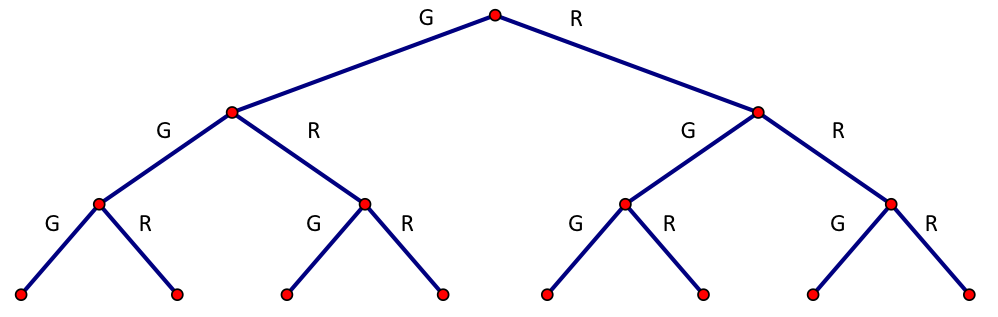
\includegraphics[scale=0.8]{tree.png}
\end{image}
\vspace{.15in}
\item What is the probability of three reds? 
\item What is the probability of two reds and a green? 
\item What is the probability of one red and two greens? 
\item What is the probability of three greens? 
\item If the first cube is green, what is the probability that the second cube is red? 
\item If the first cube is red, what is the probability that the second cube is red? 
\item What is the probability that the second cube is red?  
\end{enumerate}
\end{problem}

\newpage
\begin{problem}
Place \textbf{three green} cubes and \textbf{three red cubes} in a bag.  Without looking, draw three cubes, one at a time, \textbf{this time with replacement}.  
\begin{enumerate}
\item Write probabilities in the tree diagram below to organize the possible outcomes and compute their probabilities.  
\begin{image} 
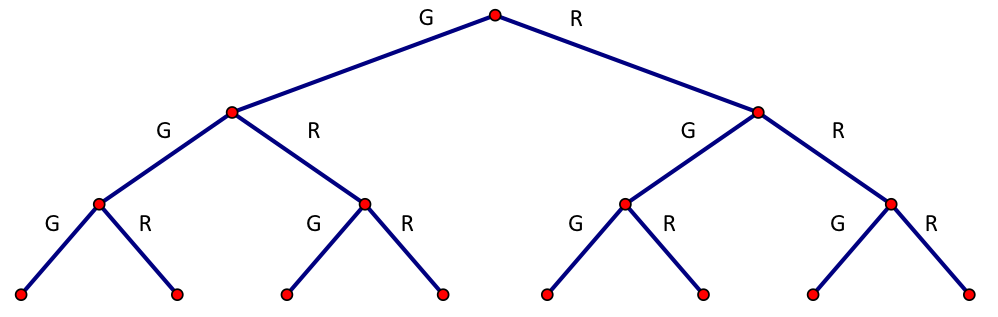
\includegraphics[scale=0.8]{tree.png}
\end{image}
\vspace{.15in}
\item What is the probability of three reds? 
\item What is the probability of two reds and a green? 
\item What is the probability of one red and two greens? 
\item What is the probability of three greens? 
\item If the first cube is green, what is the probability that the second cube is red? 
\item If the first cube is red, what is the probability that the second cube is red? 
\item What is the probability that the second cube is red?  
\item Use the words "dependent" and "independent" to contrast the probability that the second cube is red in this and the previous scenario.  
\end{enumerate}
\end{problem}

\newpage
\begin{problem}
This time, place \textbf{two green} cubes and \textbf{three red} cubes in a bag.  Without looking, draw three cubes, one at a time, \textbf{again with replacement}.  
\begin{enumerate}
\item Write probabilities in the tree diagram below to organize the possible outcomes and compute their probabilities.  
\begin{image}
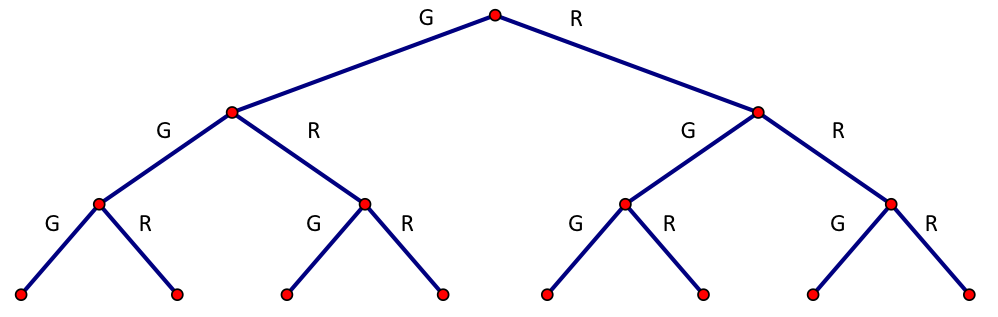
\includegraphics[scale=0.8]{tree.png}
\end{image}
\vspace{.15in}
\item What is the probability of three reds? 
\item What is the probability of two reds and a green? 
\item What is the probability of one red and two greens? 
\item What is the probability of three greens? 
\item If the first cube is green, what is the probability that the second cube is red? 
\item If the first cube is red, what is the probability that the second cube is red? 
\item What is the probability that the second cube is red?  
\item Is the probability that the second cube is red independent of the outcome of the first cube?  Explain. 
\item In the previous scenario, some outcomes are equally likely.  Is that true here?  Why or why not? 
\end{enumerate}
\end{problem}

\newpage

\begin{problem}
Suppose the Indians and the Yankees are to face each other in a best-of-three series.  Suppose the probability that the Indians will win any game is 60\%, and suppose the outcomes of the games are independent of one another.  
\begin{enumerate}
\item Draw a tree diagram for the series.  
\item What is the probability that the Indians win games 1 and 3 to win the series?
\item What is the probability that the Indians win the series in exactly 3 games?
\item What is the probability that the Indians win the series?
\end{enumerate}
\end{problem}


\begin{problem} 
Fred the Slob has an unreliable car that starts only 60\% of the days.
If the car doesn't start, poor Fred must walk the one block to work.
This week, he is slated to work 5 days (Monday through Friday).  
\begin{enumerate}
\item What is the probability that Fred will walk on Monday and Wednesday
and drive the other days?
\item What is the probability that Fred will drive on exactly 4 of the days? 
\item What is the probability that poor Fred will have to walk on at least two of the days?
\end{enumerate}
\end{problem}



%\begin{problem}
%Use the techniques of this activity (i.e., using a special case and
%fraction arithmetic to help investigate a more general case) to find
%the probability of passing a 10-question true/false test by guessing if you
%must get 70\% or more correct to pass.
%\end{problem}

\end{document}
